\chapter{Link Layer Security: noncoresec} \label{Chp: LLSEC}

In this chapter, we analysis the Link Layer security measure in Contiki, noncoresec.

One thing to be noticed is that IPv6 fragmentation may affect some packet features. However, as it would be avoided by most of the applications, we assume the packets are not fragmented in this section.

\section{Protocol and Implementation}

\cite{802154sec} has introduced some problems induced by the design of 802.15.4 security, as we has summarised in \Cref{Subsec: 802154 Sec Issue}. Since noncoresec supports only network shared key, we do not consider the key management issues mentioned in \cite{802154sec}. As a result, there are two potential problems left on our platform:

\begin{enumerate}
	\item Nonce reuse
	\item Incompatible anti replay
\end{enumerate}

In this section, we analyse the noncoresec implementation with respect to these two potential problems. The term ``broadcast'' in this section represents Link Layer broadcast.

\subsection{Nonce Reuse}

As we have explained in \Cref{Subsec: 802154 Nonce}, the only variable field in the nonce is Frame Counter. Since noncoresec only supports network shared key. Inspecting the source code, we realised that the Frame Counter is declared as a static value and therefore is initialised to $0$ on each reboot.

Our experiments confirmed the vulnerability. We simulated two executions of  broadcast\_example of keyllsec in \Cref{Sec: Applications}, broadcasting the same message. Our data\cite{NonceReuseData} showed that frames with the same Frame Counter results into the same ciphertext. In reality, this vulnerability implies that an adversary capable to reset the device can eventually learn the difference in plaintext by calculating the difference of ciphertext with the same Frame Counter, causing severe breach of data confidentiality.

One solution might be to store part of the Frame Counter on the flash and increases that value on each time reboot. Assume the device averagely sends one frame every minute stores the highest byte of Frame Counter, it is resilient in $2^8$ reboots and the lower bytes still has the space of $2^{24}$ frames, which holds up to nearly 32 years. Another solution could be to set the higher bytes of Frame Counter to a random value on each reboot. For example, by setting the highest byte to a uniformly distributed random value in $[0,255]$, the adversary is expected to successfully reset the Frame Counter to a specific value with probability of $2^{-8}$ on each reboot.

\subsection{Anti Replay}

\cite{802154sec} has pointed out that anti replay in 802.15.4 Security is incompatible with network key as the same ACL entry is shared among multiple nodes, causing confusion of Replay Counter in ACL. However, with an inspection of the source code of Contiki, we realised that the noncoresec does not suffer the same problem as the ACL is not implemented; instead, a similar data structure is added to the routing table in kernel  associated to each source address.

\section{Packet Feature Analysis}

In this section, we analyse the general packet features of WSN protected by noncoresec. We focus on the following subjects:

\begin{enumerate}
	\item Frame Size
	\item Encryption timing
\end{enumerate}

During the experiments, we also realised that the RPL messages can be distinguished in most of our applications by inspecting the MAC destination address and frame size, even though it is part of the encrypted MAC Payload.

\subsection{Frame Size} \label{noncoresec frame size}

As described in \Cref{Subsec: 802154 Sec}, when 802.15.4 Security is enabled, the MAC Frame will have an additional Auxiliary Security Header and MIC. Since no Key Strategy support is implemented and we imposed Security Level $7$ in all our related applications, it is expected that noncoresec will linearly increases the frame size as explained in \Cref{Semantic Packet Size}.

Theoretically, the value of $b$ in \Cref{Eq: Linear Length} for noncoresec is $21$, for $5$ bytes from Auxiliary Header\footnote{Security Level together with Key Strategy are aligned into $1$ byte.} and $16$ bytes from the $128$ bits MIC.

%With broadcast and unicast respectively.
Our Cooja simulation confirmed this conjecture. We have done two groups of experiments on TelosB mote simulator, one with keyllsec broadcast application and the other with unicast application.

An example data is available at: \\
\url{https://github.com/Salties/MyRepository/tree/master/experiments/keyllsec/Data/frame_size}

\subsubsection{Broadcast}
In case of broadcast without noncoresec, the relation of application data, i.e. UDP Payload, size $l_D$ and plaintext MAC Frame size $l_P$ in bytes are:
\begin{equation}
	l_D = l_{P} - 66
\end{equation}

With noncoresec enabled, the application data size $l^{\prime}_D$ and ciphertext MAC Frame size $l_C$ are:
\begin{equation} \label{Eq: broadcast llsec data size}
	l^{\prime}_D = l_{C} - 87
\end{equation}

Assuming the same application data is sent, i.e. $l_D = l^{\prime}_D$, the change of frame size induced by noncoresec is:
\begin{equation}
	b = l_C - l_P = (l^{\prime}_D + 87) - (l_D + 66) = 21
\end{equation}

\subsubsection{Unicast}

In case of keyllsec unicast application, we have:

\begin{equation}
	l_D= l_P - 80
\end{equation}

\begin{equation} \label{Eq: unicast llsec data size}
	l^{\prime}_D = l_{C} - 101 
\end{equation}

Therefore, 
\begin{equation}
	b = l_C - l_P = (l^{\prime}_D + 87) - (l_D + 66) = 21
\end{equation}

which is exactly the expected value.

\subsubsection{Conclusion}

In either cases, the size of additional data induced by noncoresec is $21$ bytes. Specifically, \Cref{Eq: broadcast llsec data size} and \Cref{Eq: unicast llsec data size} can be used to deduce the application data size in frames protected by noncoresec.

\subsection{Encryption Timing}

\subsection{RPL Messages}

ICMPv6 messages are used for IPv6 network maintenance. Specifically, RPL messages are a family of ICMPv6 messages those are directly responsible in forming and maintaining a 6LoWPAN network. 

ICMP messages are solely handled by the Contiki kernel and are thus transparent to  upper layer applications. Some of them, including RPL messages, are generated spontaneously by the Contiki kernel even when no application is running. We observed three RPL messages in our experiments, which are DIS, DIO and DAO. Four ICMPv6 messages are also observed, namely NS, NA and Echo messages. The semantic of these ICMPv6 messages are described in \Cref{Subsec: ICMPv6}.

Further more, we realised all these ICMPv6 messages has distinctive packet features with respect to the combination of packet size and destination address family. We summarise the packet features in \Cref{Tbl: Packet Features of ICMPv6 Messages in 6LoWPAN with noncoresec}, where ``0xffff'' is the Link Layer broadcast address.

\begin{table}[ht!]
	\center
	\begin{tabular}{|c|c|c|}
		\hline
		       & Packet Size (bytes) & 802.15.4 Destination Address \\ \hline
		DIS    & 85                  & 0xffff                       \\ \hline
		DIO(1) & 118                 & 0xffff                       \\ \hline
		DIO(2) & 123                 & unicast                      \\ \hline
		DAO    & 97                  & unicast                      \\ \hline
		NS (1) & 87                  & 0xffff                       \\ \hline
		NS (2) & 87                  & unicast                      \\ \hline
		NA     & 87                  & unicast                      \\ \hline
		ECHO   & 112(*)               & unicast                      \\ \hline
	\end{tabular}
	\caption{Packet Features of ICMPv6 Messages in 6LoWPAN with noncoresec, where 0xffff is the Link Layer broadcast address.}
	\label{Tbl: Packet Features of ICMPv6 Messages in 6LoWPAN with noncoresec}
\end{table}


\paragraph{Explanation of \Cref{Tbl: Packet Features of ICMPv6 Messages in 6LoWPAN with noncoresec}}
\begin{enumerate}
	\item DIO and NS message can be sent in either multicast or unicast. The broadcast DIO message is smaller than the unicast one as it uses an abbreviated IPv6 multicast address ``ff02::1a''. NS uses another multicast destination address, ``ff02::1:ff00:0'', which has the same length as an unicast address. However, both of them are translated to the same ``ffff'' Link Layer broadcast address in 802.15.4 MAC Header.
	%ICMP ECHO fragmentation in Wismote network.
	\item The size of ICMP ECHO Request and Response may vary due to its payload. On our host machine which runs on Ubuntu 15.04, the default ping command payload is 56 bytes which is expected to result into a frame of 157 bytes, exceeding the MTU required by \cite{802154} and causes fragmentation. The ``-s'' option is therefore used to reduce the size of ICMP ECHO packets. Theoretically, any packet less than 802.15.4 MTU, i.e. 127 bytes, should not be fragmented; however, in our experiments, we realised that ICMP ECHO packets larger than $107$ bytes, i.e. with payload more than $6$ bytes, will be fragmented. We have not identified the exact reason but we consider this might be a bug of implementation.
	%No NS and NA in Sky network.
	\item Different ICMPv6 messages maybe observed on different platforms. In our experiments, there is no NS and therefore NA observed in WSN built with TelosB.
\end{enumerate}

%Less than minimum size ICMP.
Recall \Cref{Eq: broadcast llsec data size} and \Cref{Eq: unicast llsec data size}, when at least one byte is sent, the minimum frame sizes are 88 bytes and 102 bytes for broadcast and unicast respectively; therefore packets with size less than these values can be immediately categorised as non application packets, which are basically ICMPv6 messages in practice. Some ICMPv6 messages are thus can be distinguished, as shown in \Cref{Tbl: Distinguishable ICMP Messages}.

\begin{table}[ht!]
	\centering
	\begin{tabular}{|c|c|}
		\hline
		$<\text{Frame Size}, \text{Destination Address}>$                     & ICMPv6 Message \\ \hline
		\textless85, broadcast\textgreater & DIS            \\ \hline
		\textless87, broadcast\textgreater & NS             \\ \hline
		\textless97, unicast\textgreater   & DAO            \\ \hline
		\textless87, unicast\textgreater   & NS / NA        \\ \hline
	\end{tabular}
	\caption{Distinguishable ICMP Messages}
	\label{Tbl: Distinguishable ICMP Messages}
\end{table}

%NS & NA, DIS & DIO
NA is only sent as a response to NS; therefore if a round trip of two 87 bytes unicast packet, it is likely that the first one is NS and the second NA. Similarly, DIS is sent for requesting DIO messages.  Once a valid DIO is received, the node no longer sends out DIS. Therefore if a sequence of broadcasted 85 bytes frames is terminated by a frame of 118 bytes, they are likely to be DIS and DIO messages.

Other ICMPv6 messages are still possible to be distinguished by \Cref{Tbl: Packet Features of ICMPv6 Messages in 6LoWPAN with noncoresec}, but misidentification may occur if the application happened to send packets of both same size and destination address.

%Full list of ICMP

%Example Data
Example data are available at:\\
\url{https://github.com/Salties/MyRepository/tree/master/experiments/keyllsec/Data/RPL}

%Sequence Numbers
%No need to do this any more...
%\section{Application Analysis}

%\section{Packet Forwarding}



%
%Link Layer Security, or LLSEC, is a security measure that implements cryptography at Data Link Layer\footnote{https://en.wikipedia.org/wiki/OSI\_model} which is only above Physical Layer.
%
%Introducing cryptography at a lower level has several benefits. Firstly, more data being encrypted reduces the observable packet features to an adversary, such as SRC\footnote{Source Address} and DST\footnote{Destination Address} field in the IP header which are very likely to be exploited by an adversary. Secondly, authentication at lower level also prevents an active adversary from joining the network which therefore weakens her power. 
%
%On the other hand, imposing cryptography at a lower level also brings more challenge to the design of sensor network architecture. The first problem is its overhead. For example, even for a node that only forwards a packet to its next hop, it must decrypt the whole packet to extract its routing information, and then re-encrypt it before transmission. This is particularly problematic in a mesh wireless sensor network as it could potentially downgrades the performance and causing energy consumption problems. More over, key management is also challenging due to the constrained computational power and power optimised lossy nature of wireless sensor network.
%
%It is noticeable that some packet features are not hidden even with LLSEC enabled, such as packet length, timing information and part of the MAC header in a 802.15.4 packet.
%
%\section{802.15.4 Security: {\it noncoresec}} \label{sec: noncoresec}
%{\it noncoresec}\cite{LLSEC} is the current implementation of LLSEC in Contiki. It implements AES\_CCM\_16 ciphersuite in 802.15.4 standard. This section briefly describes how it works.
%
%\begin{itemize}
%\item {\bf Key Management}: All nodes share a network wide AES key for both encryption and authentication. The key is hardcoded during the setup stage.
%
%\item{\bf AEAD\footnote{Authenticated Encryption with Associated Data}}: {\it noncoresec} implements AES\_CCM\_16 \footnote{CCM mode of AES-128 with 16 bytes MAC} as described in 802.15.4\cite{802154} which turns AES into a stream cipher. The same key is used for both encryption and authentication.
%
%\item{\bf Initial Vector (IV, or nonce)}: The IV for each packet is constructed from certain fields of unencrypted MAC header and therefore is public.
%\end{itemize}
%
%An adversary without the knowledge cannot join the sensor network protected by \textit{noncoresec} as she cannot sent out a valid RPL message.
%
%\section{Weak IV}
%
%\begin{figure}
%\centering
%\begin{tabular}{| l | l | l | l | l |}
%\hline
%Flags(1) & Addresses(8) & Frame Counter(4) & Security Level(1) & Block Counter(2)       \\ \hline
%\end{tabular}
%\caption{IV of 802.15.4 Frame with Security} \label{Tbl: 802154 Frame}
%\end{figure}
%
%One problem within the {\it noncoresec} implementation is the low variance of IV. The IV is a $16$ byte bit-string constitutes of the following fields(\Cref{Tbl: 802154 Frame}):
%\begin{itemize}
%\item {\bf Flags (1 byte)}: This field contains part of the MAC header. It is identical to most (basically all) of the data packets.
%
%\item{\bf Source Address (8 bytes)}: This is mapped from the source address field of the packet.
%
%\item{\bf Frame Counter (4 bytes)}: This field increases by 1 from 0 for each packet sent to prevent replay attack.
%
%\item{\bf Security Level (1 byte)}: This field indicates which ciphersuite to be used for this packet. In the case of AES\_CCM\_16, this is constantly 0x7.
%
%\item{\bf Block Counter (2 bytes)}: This field begins from 0x0 and increases by 0x1 for each block in CCM mode. The block length for AES-128 is 16 bytes. The 2 bytes counter is usually sufficient as it supports up to $2^{32}$ bytes of data whereas the minimum MTU\footnote{Maximum Transmit Unit, simply speaking this is the maximum length of a packet.} required by 6lowPAN standard\cite{rfc4944} is $127$ bytes.
%\end{itemize}
%
%In the current {\it noncresec} implementation, \textbf{Flags} and \textbf{Security Level} are constant. \textbf{Block Counter} always begins from 0x0 and the \textbf{Source Address} is also constant for a specific device. Such design leaves the 4 bytes \textbf{Frame Counter} the only field that is variable. This indicates that only $2^{32}$ messages are allowed without a collision of IV which is cryptographically considered to be inappropriate.
%
%\subsection{Reset Problem}
%The low variance of IV leads to a plaintext leakage problem which only requires the adversary to reboot the target node. 
%
%The idea is that rebooting the device resets the \textbf{Frame Counter} to 0x0; hence once a pair of packets with same \textbf{Frame Counter} is found, the difference of their plaintext can be computed by their ciphertext:
%\begin{equation*}
%\Delta p = c_1 \oplus c_2
%\end{equation*}
%where $\Delta p$ is the difference of plaintexts. $c_1$ and $c_2$ are their ciphertext respectively.
%
%\begin{example}
%\begin{figure*}
%\centering
%{
%	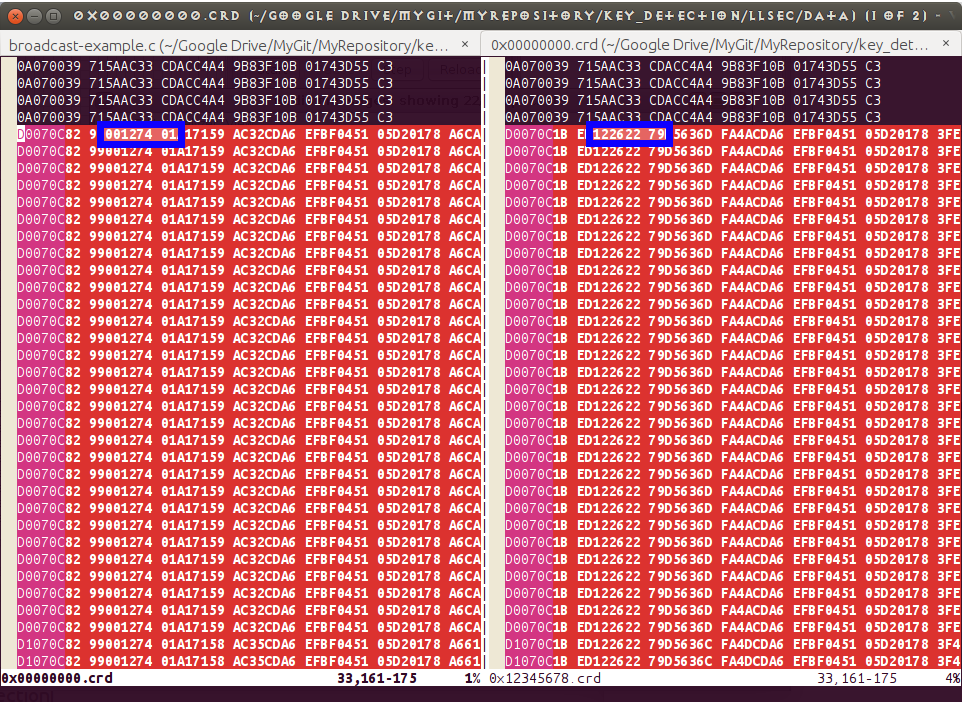
\includegraphics[width=0.9\textwidth,]{fig/resetproblem.png} 
%}
%\caption{Captured packets with {\it noncoresec} enabled} \label{Fig: reset problem}
%\end{figure*}
%
%\Cref{Fig: reset problem} demonstrates some packet captured\footnote{The duplicated packets are caused by the retransmission of ContikiMAC\cite{ContikiMAC}.} with {\it noncoresec} enabled. These packets are captured with a sensor broadcasting a 4 byte integer with left side of \Cref{Fig: reset problem} being $[00000000]_{16}$ and right $[12345678]_{16}$. Marked are the corresponding ciphertexts which are $[00127401]_{16}$ and $[12262279]_{16}$ respectively.
%
%As we can see, the difference of ciphertext is exactly the difference of plaintext:
%\begin{equation}
%\Delta p = [00127401]_{16} \oplus [12262269]_{16} = [12345678]_{16}
%\end{equation}
%\end{example}
%
%\section{Distinctive Packet Length for RPL Packets}
%Some RPL packets are shorter than the minimum length of data packets which can be used to distinguish the packets. Further more, some RPL packets set MAC header flags differently from data packets.
%
%\section{Performance Issue}
%The header overhead with LLSEC enabled is 20 bytes which is relatively a large overhead comparing to the 127 bytes MTU requirement of 6LowPAN standard\cite{rfc4944}.